{% -*- mode: LaTeX; TeX-PDF-mode: t; TeX-master: "manual"; -*-
}

\chapter{\ei Clients}
\label{ch:clients}


\section{Web-Client}
\label{ch:clients:web}

\begin{figure}[t]
\hrule\smallskip
\begin{center}
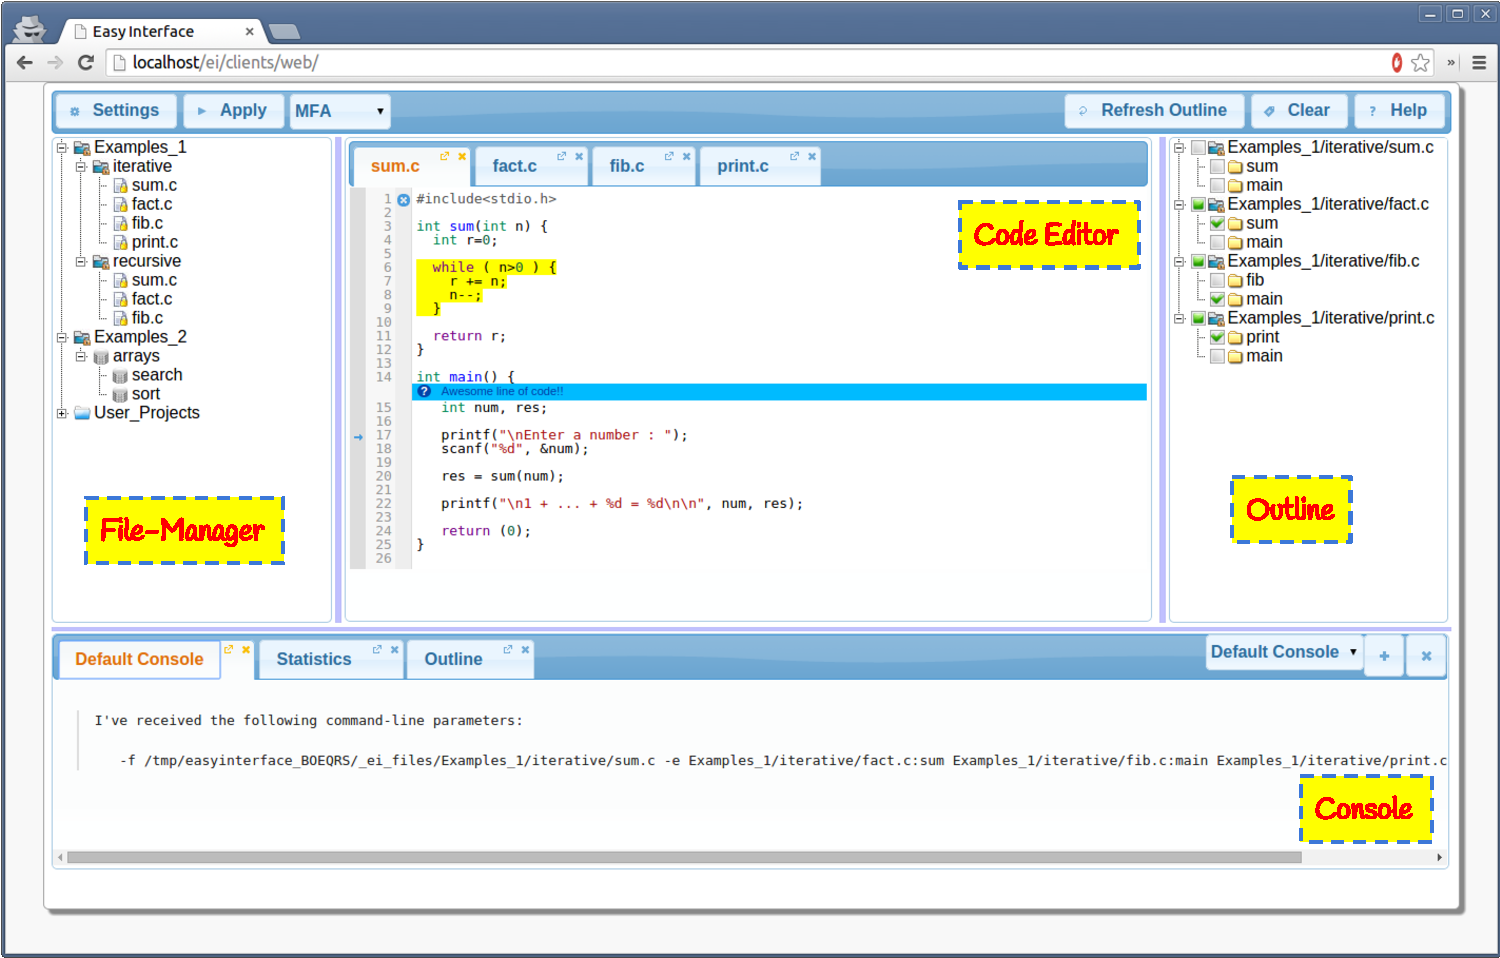
\includegraphics[width=1\textwidth]{fig/webclient.pdf}
\end{center}
\caption{\ei Web Client}
\label{fig:webclient}
\hrule
\end{figure}


\subsection{Generate Outline}
\label{ch:clients:web:outline}

The Outline App returns an XML with the outline tree.

%% 
\bigskip
\xmlstruct
{outline}
{
%
  Defines a list of points to be analysed.
\begin{itemize}
  \item \xmlstructattr{text} is the name to be show.
   \item \xmlstructattr{value} is the internalname .
\item \xmlstructattr{selectable} indicates if this node can be
  selected.
\item \xmlstructattr{icon} indicates an alternative path for the icon
  of the node.

\end{itemize}
%
}
{\xmlstructrefwb{outline}}




\section{Eclipse Plugin}
\label{ch:clients:eclipse}

\section{Remore shell}
\label{ch:clients:shell}
